\chapter{Semantic Assertions for Interconnecting Provenance Elements of Research Publications}
\label{ch:ontologies}
\section{PROV-PUB-O/S specifications}
The design of PROV-PUB-O/S follows a minimalist approach on class definitions to make a small ontology just sufficient for the purpose of describing the results and the parts of the research publications that contain them. Figure~\ref{fig:prov-pub-s-classes} and Figure~\ref{fig:prov-pub-s-properties} shows the classes and properties in PROV-PUB-O/S, respectively.

\begin{figure}
	\centering
	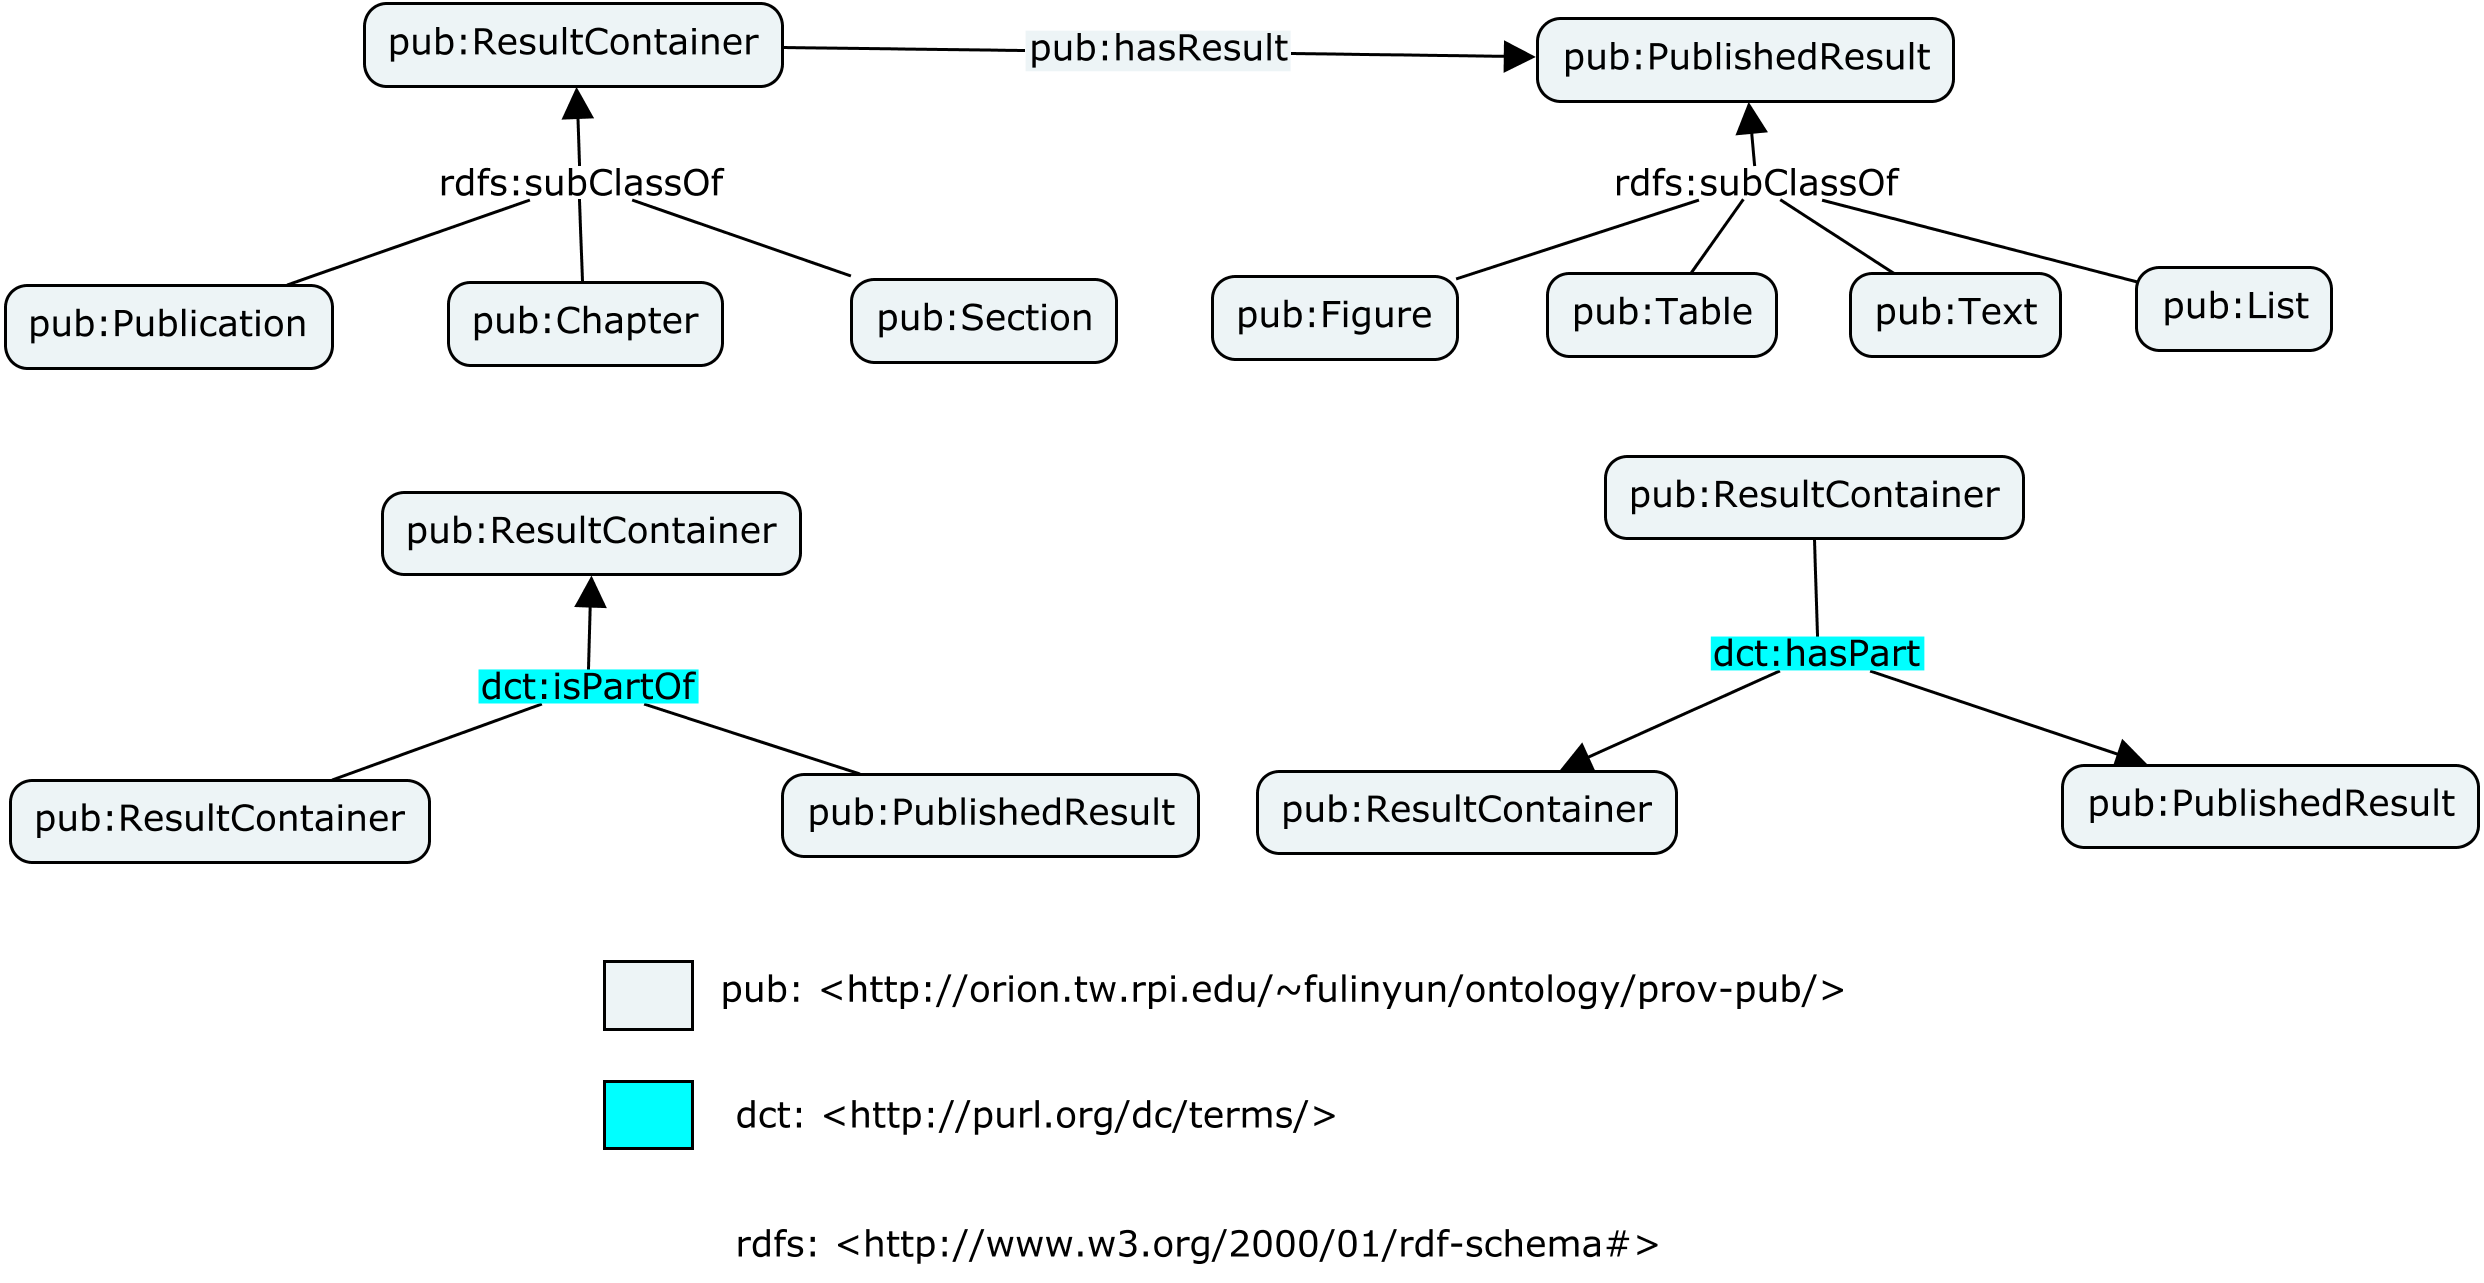
\includegraphics[width=\textwidth]{model/ontology/prov-pub/prov-pub-s-classes.png}
	\caption{Classes in PROV-PUB-O/S}
	\label{fig:prov-pub-s-classes}
\end{figure}

\begin{figure}
	\centering
	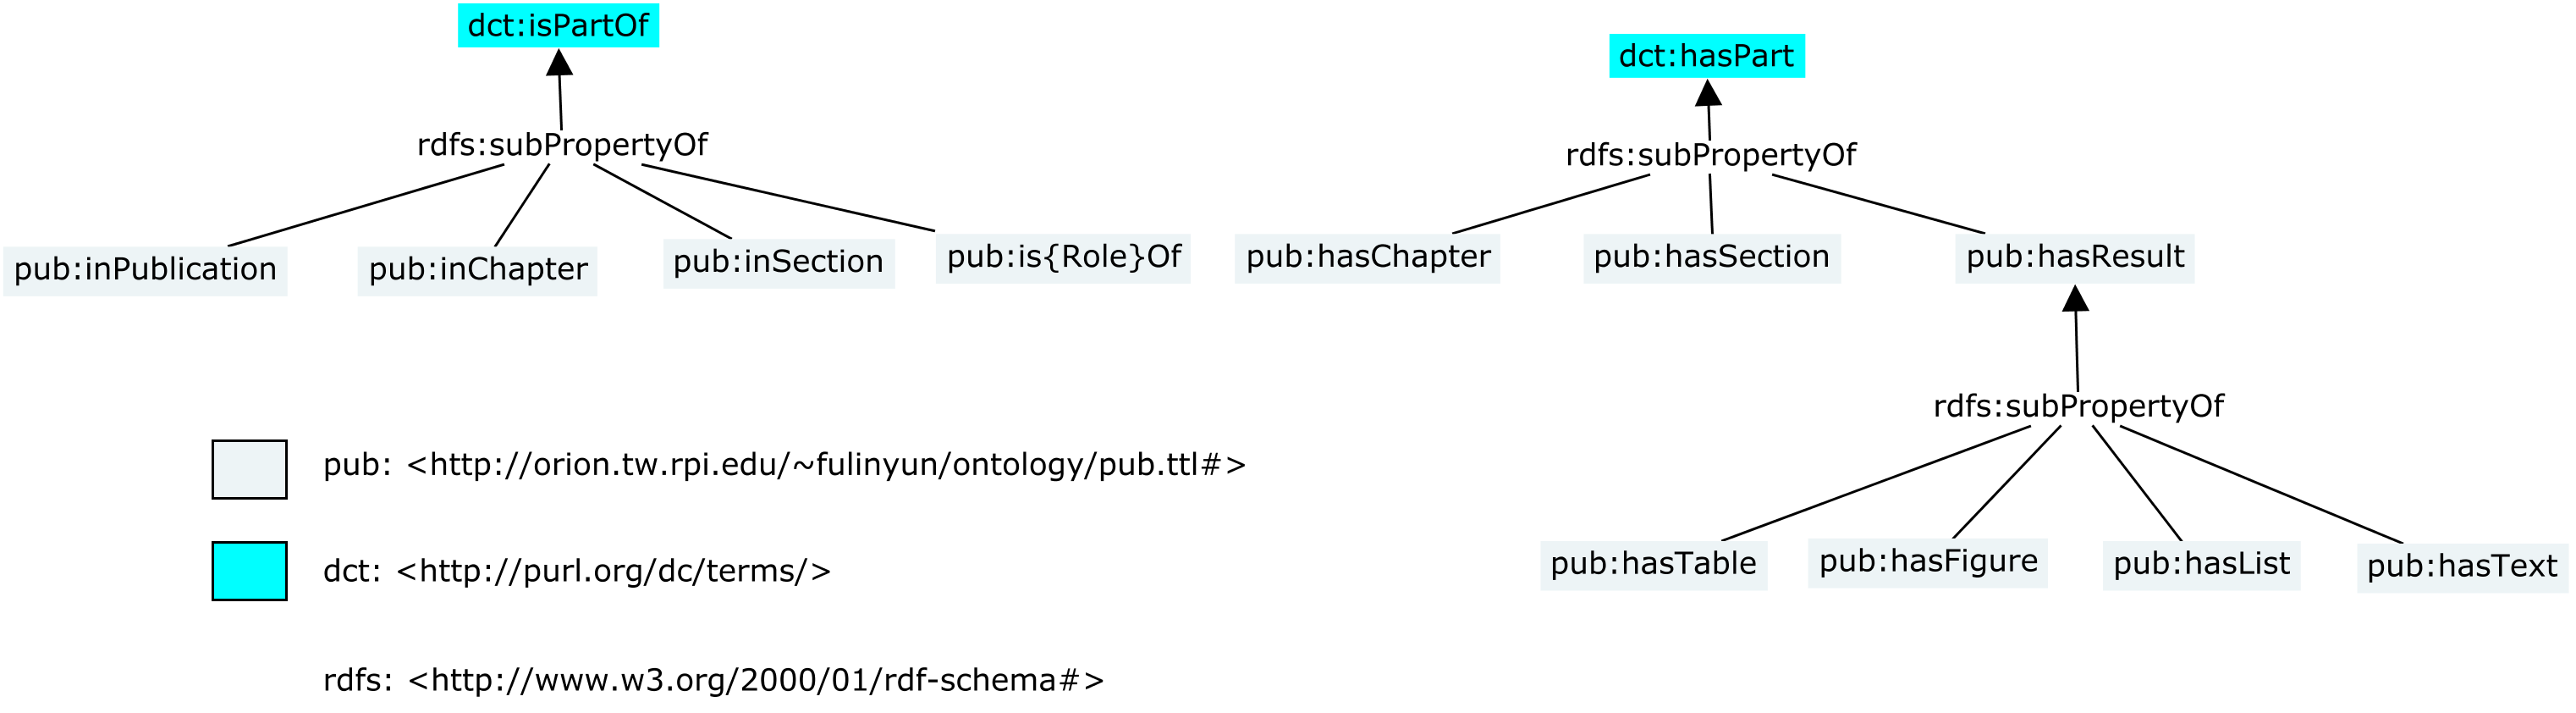
\includegraphics[width=\textwidth]{model/ontology/prov-pub/prov-pub-s-properties.png}
	\caption[Properties in PROV-PUB-O/S]{Properties in PROV-PUB-O/S, where pub:is{Role}Of represents the role indicating properties such as pub:isIntroductionOf, pub:isAbstractOf, and so on}
	\label{fig:prov-pub-s-properties}
\end{figure}


An important conceptual deviation of PROV-PUB-O/S from DoCO is that in DoCO, tables and figures are considered blocks of documents the same way as chapters and sections, but in PROV-PUB-O/S, they are considered research results instead of normal document parts. Other block elements such as chapters and sections are also considered result containers in PROV-PUB-O/S. They are defined to serve the function of locating interesting results in research publications. We stop our document part modeling at the section level because sections are the most fine-grained elements that have (numerical) labels such as ``Section 2.1.1'' and/or captions such as ``PROV-PUB-O/S: publication structure modeling''. This is not the case for paragraphs and sentences. Note that subsections of a section is also instances of pub:Section. 
%Minimalism here means to only define a set of ontology elements that must be defined together to ensure their proper function, so PROV-PUB-O/S does not 
%assert any of its classes to be a subclass or equivalent class of a class from another ontology if that assertion is not necessary for PROV-PUB-O/S to 
%function properly.

Four types of published results are defined in PROV-PUB-O/S: tables, figures, lists and textually described results. 

PROV-PUB-O/S can also be used together with the BibTeX ontology\footnote{The BibTeX ontology: \url{<http://purl.org/net/nknouf/ns/bibtex>}, accessed on October 10th, 2015.} or the Bibliographic Ontology\footnote{The Bibliographic Ontology: \url{<http://purl.org/ontology/bibo/>}, accessed on October 10th, 2015.}. Since no subclassing link to the related ontologies is hard coded in PROV-PUB-O/S, the users have the choice of whether 
to link PROV-PUB-O/S with these three ontologies (and thus depend on them) and to what extent. 

Two typical ways of linking PROV-PUB-O/S with its related ontologies are subclassing and double-classing. Subclassing means to assert that a class in PROV-PUB-O/S is a subclass of 
a class in one of the related ontologies. For example, the user could optionally assert that pubs:Chapter is a subclass of 
doco:Chapter to make every instance of pubs:Chapter automatically also an instance of doco:Chapter. Double-classing means to assert that an instance of 
a PROV-PUB-O/S class is also an instance of another class in a related ontology. For example, an instance can be asserted as both a pubs:Publication 
and a bibo:Document.

Following the principle of ``Leaving the decision for dependencies to the users'', mentioned at the beginning of this section, subclassing and double-classing suggestions are given for each class in PROV-PUB-O/S 
in case the user of the ontology 
wants to reuse the classes and constraints defined in the related ontologies.

Three bridging 
ontologies\footnote{Like PROV-PUB-O itself, these bridging ontologies are not officially published yet, and are temporarily hosted at \url{http://orion.tw.rpi.edu/~fulinyun/ontology/prov-pub/prov-pub-s-doco.ttl}, \url{http://orion.tw.rpi.edu/~fulinyun/ontology/prov-pub/prov-pub-s-bibtex.ttl} and 
	\url{http://orion.tw.rpi.edu/~fulinyun/ontology/prov-pub/prov-pub-s-bibo.ttl}, accessed on October 10th, 2015.} are provided in case a user wants to accept all the suggested subclassing links from
PROV-PUB-O/S to one of its related ontologies. Each bridging ontology is exclusively composed of assertions of the form ``pubs:X rdfs:subClassOf doco:Y'' 
such as ``pubs:Chapter rdfs:subClassOf doco:Chapter''. Double-classing suggestions cannot be encoded in the form of bridging ontologies because they do 
not require any assertion at the schema level.

There are existing ontologies, such as the GCIS ontology \cite{ma2014ontology}, that also have classes to represent document components such as chapters, but we prefer not reusing from such application ontologies because PROV-PUB-O/S is considered to be a general ontology for all kinds of research publications, and it is logical to have application ontologies make subclassing and/or equivalent-classing assertions to general or domain ontologies, but not the other way around.

The PROV-PUB-O ontology, the three bridging ontologies, and usage examples of PROV-PUB-O can be found in Appendix~\ref{ap:ontologies}, all serialized in Turtle.

\section{PROV-PUB-O/P specifications}
Based on the principles of minimalism on classes, rich on properties and leaving the decision for dependencies to the users, as well as the semiotic framework and the case study mentioned in Section~\ref{subsec:process}, we define the following classes and properties in PROV-PUB-O/P:

{\noindent\emph{Classes about data:}}
\begin{itemize}
	\item pub:Data
	\item pub:InMemoryData
	\item pub:OnDiskData
\end{itemize}
We define pub:Data as a subclass of prov:Entity, and pub:InMemoryData and pub:OnDiskData are defined as subclasses of pub:Data. They represent data residing in memory and on disk, respectively.
{\noindent\emph{Classes about data generation:}}
\begin{itemize}
	\item pub:DataGeneration
	\item pub:PhysicalChange
	\item pub:SyntacticalChange
	\item pub:SemanticalChange
	\item pub:Obtaining
	\item pub:Loading
	\item pub:Saving
	\item pub:Transformation
	\item pub:Library
\end{itemize}
The pub:DataGeneration class is defined as a subclass of prov:Entity and is the most general class representing data generation activities. 

Semiotic framework based subclasses of pub:DataChange follows, that is, pub:PhysicalChange, pub:SyntacticalChange and pub:SemanticalChange, which we have already described earlier. 

The next four classes, pub:Obtaining, pub:Loading, pub:Saving and pub:Transformation, are derived from the case study we have performed (see Chapter~\ref{ch:case-study} for details). The pub:Obtaining class represents data obtaining activities. Subclasses conforming naming conventions of specific domains are expected to get defined in extensions of PROV-PUB-O/P. In the earth science domain, for example, a ``Download'' subclass of pub:Obtaining would probably receive common acceptance. The pub:Obtaining class could be asserted as a subclass of pub:PhysicalChange and/or pub:SyntacticalChange according to application specific conditions. The pub:Loading class represents data loading activities that read data from disk to memory. This class should probably be asserted as a subclass of both pub:PhysicalChange and pub:SyntacticalChange, but we did not put these assertions in PROV-PUB-O/P because these assertions still might be undesirable in some use cases. The pub:Transformation class represents all general data transformation activities. Subclasses conforming naming conventions in various domains are expected to get defined in extensions of PROV-PUB-O/P. For example, ``subsetting'', ``slicing'', ``projection'' and ``filtering'' are four transformations commonly used in the earth science domain.

The last class listed above, pub:Library, represents those software utilities or tools used in the process of generating data and results. The detailed information about the software could be described with a software description ontology such as the OntoSoft ontology \cite{gil2015ontosoft}.

Users are expected to either define subclasses of these data changing activities to fit their specific needs or overlook the subclasses of pub:DataChange and pub:ResultGeneration. That is, they could extend PROV-PUB-O/P with more data changing subclasses such as ``subsetting'', ``slicing'', ``projection'' and ``filtering'', or if they do not need classes so specific, they could just use pub:DataChange to capture every data changing activities involved in their use cases.

\noindent\emph{Classes about result generation:}
\begin{itemize}
	\item pub:ResultGeneration
	\item pub:Visualization
	\item pub:Analysis
	\item pub:Reuse
\end{itemize}
These four classes represent the general result generation activity and three general ways of result generation, namely visualization typically used to create figures, analysis typically used to create tables, lists and textually described results, and reuse that generate a new result by reusing an existing one. The latter three are all subclasses of the first.

We define change of data as an activity that used data to generate data, and result generation as an activity that used data to generate results.

The pub:Library class are also likely to be used by result generation activities. We just do not list it here to avoid duplication.

Just like the classes about data generation, users are expected to either extend this part by defining more specific subclasses or overlook the two subclasses and just use pub:ResultGeneration according to their needs.

Figure~\ref{fig:prov-pub-p-entity} and Figure~\ref{fig:prov-pub-p-activity} show the extensions on prov:Entity and prov:Activity in PROV-PUB-O/P, respectively.
\begin{figure}
	\centering
	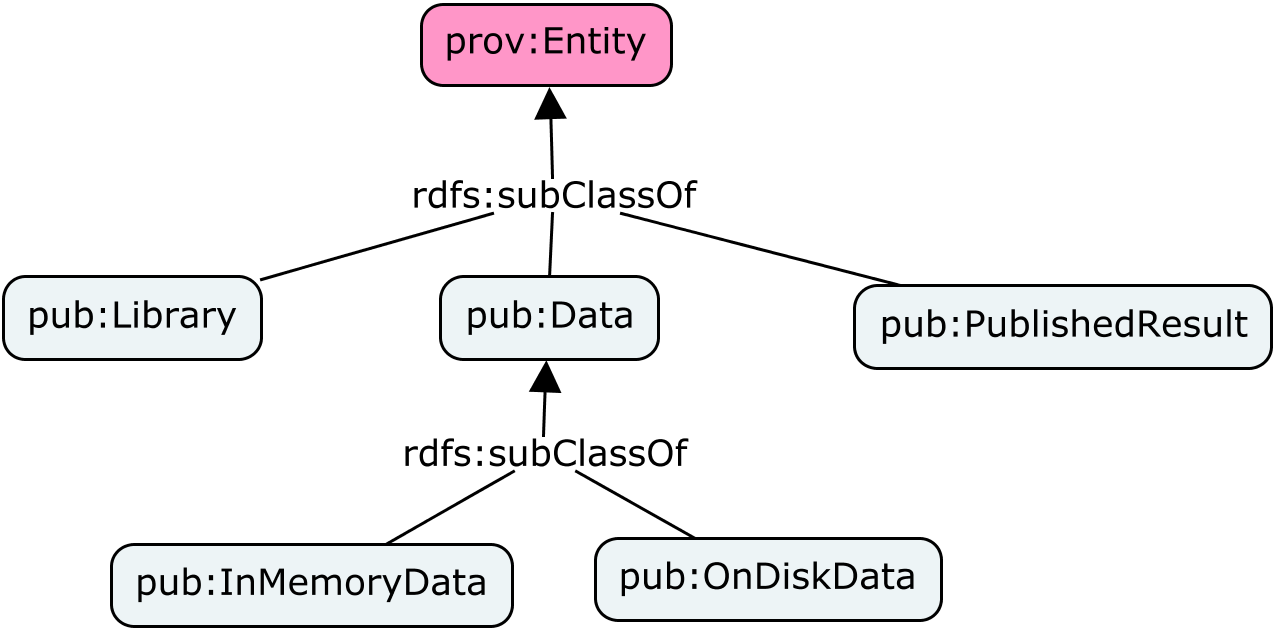
\includegraphics[width=.8\textwidth]{model/ontology/prov-pub/prov-pub-p-entity.png}
	\caption{Entities defined in PROV-PUB-O/P}
	\label{fig:prov-pub-p-entity}
\end{figure}
\begin{figure}
	\centering
	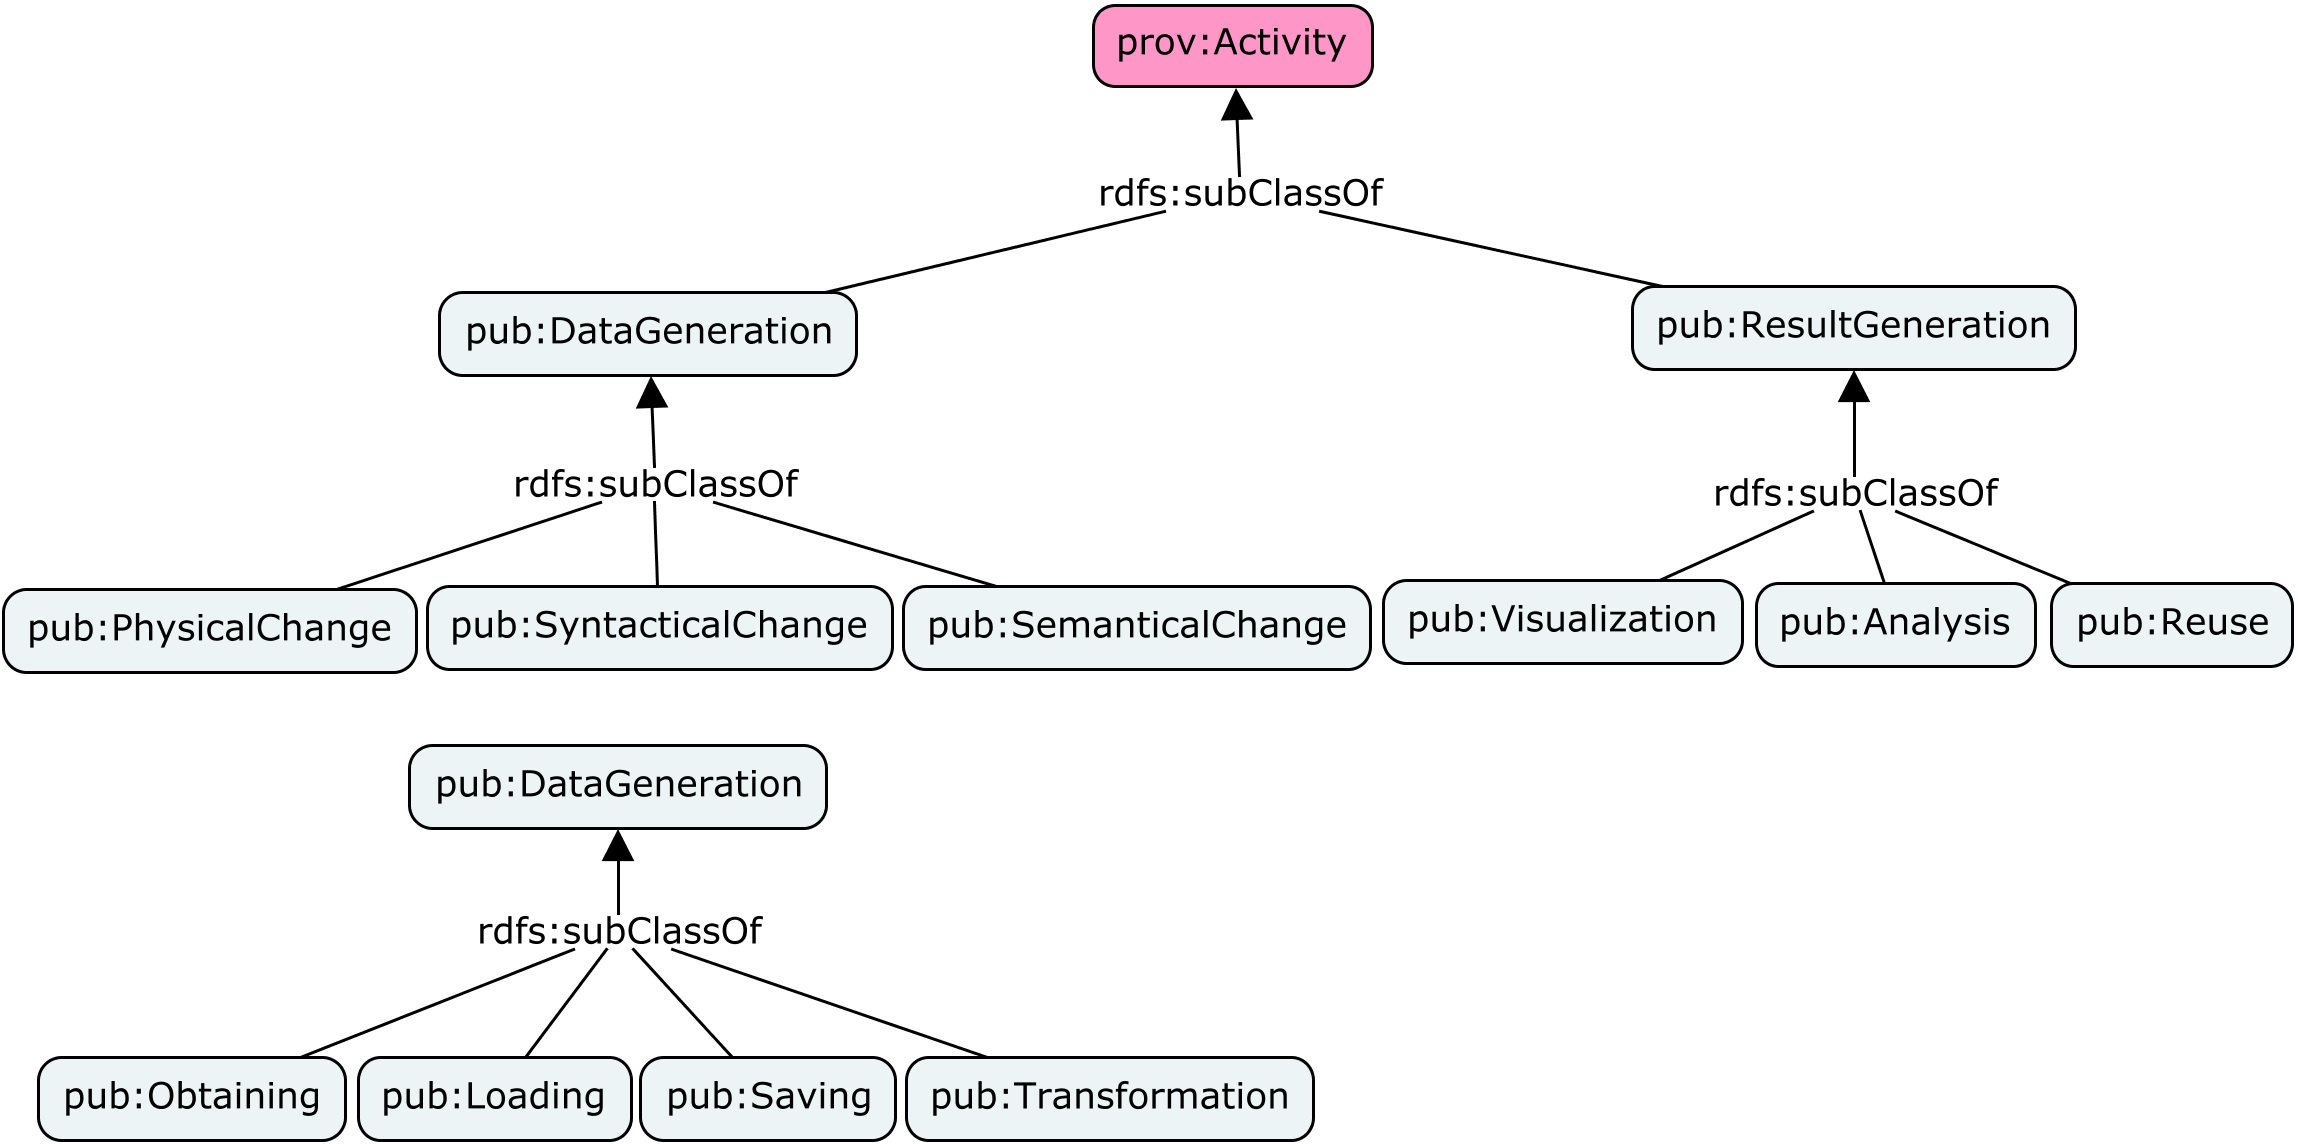
\includegraphics[width=\textwidth]{model/ontology/prov-pub/prov-pub-p-activity.png}
	\caption{Activities defined in PROV-PUB-O/P}
	\label{fig:prov-pub-p-activity}	
\end{figure}

{\noindent\emph{Properties about using data and results:}}
\begin{itemize}
	\item pub:obtained
	\item pub:loaded
	\item pub:saved
	\item pub:transformed%subset slice project filter map...
	\item pub:visualized
	\item pub:analyzed
	\item pub:reused
\end{itemize}
These are sub-properties of prov:used to allow domain-specific ways of describing data and result usage methods. Their names indicate the correspondence between these properties and the data changing and result generation activities mentioned above. For example, pub:obtained is expected to be used with the pub:Obtaining activity. These properties can also be considered ``shortcuts'' to replace the use of prov:qualifiedUsage. For example, the following usage written in PROV-O
\begin{quotation}
	:activity1 prov:qualifiedUsage [
	
	\hspace{2em}prov:entity :data1;
	
	\hspace{2em}dcterms:description "transform"
	
	].
\end{quotation}
could be written in PROV-PUB-O/P as
\begin{quotation}
	:activity1 pub:transformed :data1.
\end{quotation}
Figure~\ref{fig:prov-pub-p-usage} shows the sub-properties of prov:used that are defined in PROV-PUB-O/P.
\begin{figure}
	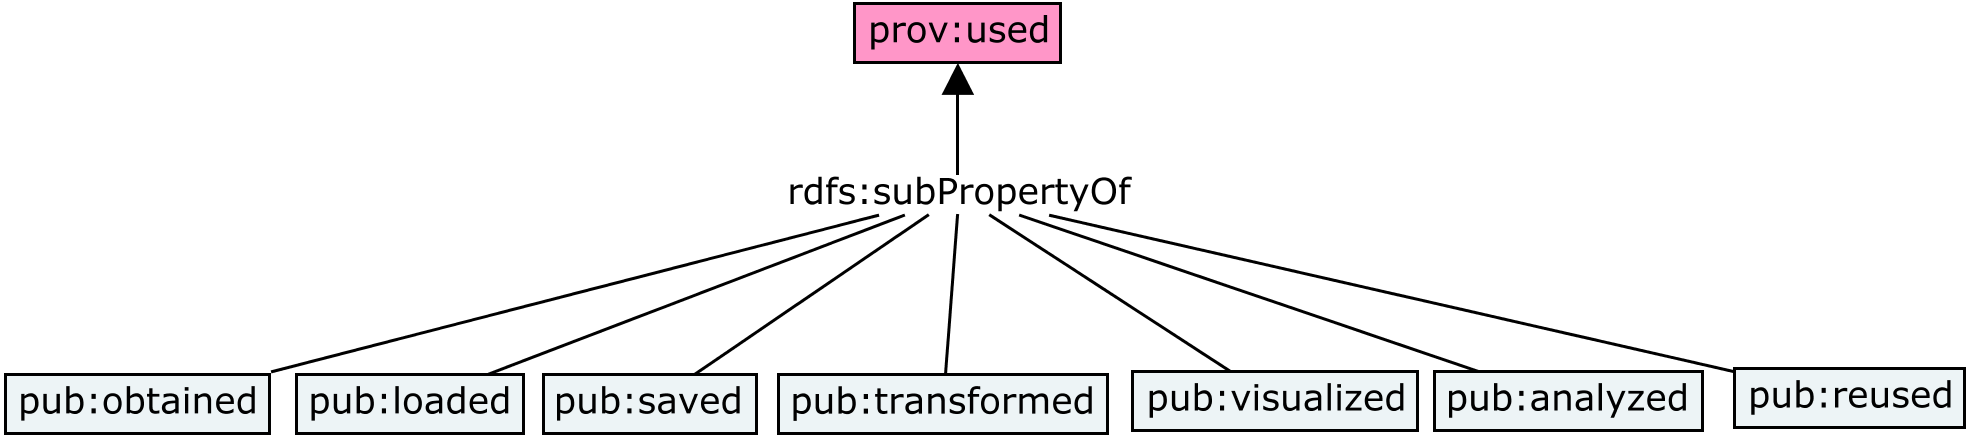
\includegraphics[width=\textwidth]{model/ontology/prov-pub/prov-pub-p-usage.png}
	\caption{Sub-properties of prov:used defined in PROV-PUB-O/P}
	\label{fig:prov-pub-p-usage}
\end{figure}

\noindent\emph{Annotations about change of data and result generation:}
\begin{itemize}
	\item pub:format
	\item pub:language% --- the programming language used in the data changing activity.
	\item pub:code% --- the code in a certain programming language for changing the data. It is recommended that only succinct code that invokes helper functions are included, and the detailed implementation of these helper functions be modeled as pub:Library instances used by data changing activities.
	\item dcterms:description% --- the textual description of the data processing method. 
\end{itemize}
These four annotations are used to describe 1) the format in which on-disk data are, 2) the programming language used in a certain data changing or result generation activity, 3) the code in a certain programming language for changing the data or generating the result and 4) the data processing method in natural language. For the pub:code annotation, it is recommended that only succinct code that invokes helper functions are included, and the detailed implementation code of these helper functions be modeled as pub:Library instances used by the activity in question.

We believe users of PROV-PUB-O/P will benefit from dependencies to PROV-O in forms of subclasses and sub-properties --- after all, this is the very reason we design PROV-PUB-O/P as a specialization of PROV-O --- so we include these assertions in PROV-PUB-O/P.

The specialized ontology is not only helpful in describing the provenance, but it also enables the construction of executable provenance graphs to preserve the data product preparing process at a level that is detailed enough for reproduction.

The PROV-PUB-O/P ontology, as well as its usage examples, can be found in Appendix~\ref{ap:ontologies}, all serialized in Turtle.

